\chapter{Introduction to DUNE}
\label{ch:exec-overall}


%%%%%%%%%%%%%%%%%%%%%%%%%%%%%%%%%%%%%%%%%%%%%%%%%%%%%%%%%%%
\section{}
\label{sec:exec-overall-1}

Sample figure to copy and edit, Figure~\ref{fig:map}:

\begin{dunefigure}[DUNE collaboration global map]{fig:mhexec}{The international DUNE
collaboration. Countries with DUNE membership are shown in orange.}
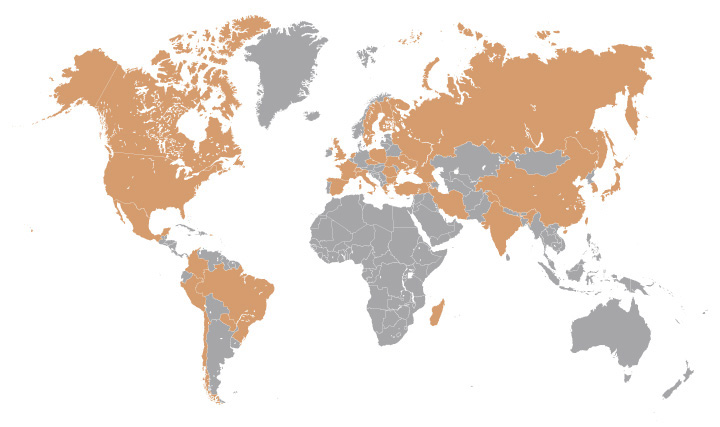
\includegraphics[width=0.9\textwidth]{global-retouched.jpg}  
\label{fig:map}
\end{dunefigure}

Sample table to copy and edit, Table~\ref{tab:execosctable}:

\begin{dunetable}[Required exposures to reach oscillation physics
  milestones]{lcc}{tab:execosctable}{The exposure in mass (kt) $\times$ proton beam power
    (MW) $\times$ time (years) and calendar years assuming the staging plan described in this chapter needed to reach certain oscillation physics
    milestones. The numbers are for normal hierarchy using the NuFit 2016 best fit values of the known oscillation parameters.  }
Physics milestone & Exposure  & Exposure \\ \rowtitlestyle
  & (\ktMWyr{}) & (years)  \\ \toprowrule 
  $1^\circ$ $\theta_{23}$ resolution ($\theta_{23} = 42^\circ$) & 29  &  1\\ \colhline
  CPV at $3\sigma$ ($\delta_{\rm CP} = -\pi/2$)  & 77 &  3\\ \colhline
  \dword{mh} at  $5\sigma$ (worst point) & 209 & 6 \\ \colhline
  $10^\circ$ $\delta_{\rm CP}$ resolution ($\delta_{\rm CP} = 0$) & 252 & %5 
  6.5 \\ \colhline
  ($\sin^2 2 \theta_{13} = 0.084 \pm 0.003$) &  &  \\  
\end{dunetable}

%%%%%%%%%%%%%%%%%%%%%%%%%%%%%%%%
\subsection{}
\label{sec:exec-overall-2}